% Section: Decisions

This section describes main decisions that were made during the development process.

\subsection{Fully-automatic or Semi-automatic Processing}
\label{ssec:processing}

Although automatic recognition can achieve very good results, there are many
sensitive areas where it is necessary to eliminate all errors, such as
police reports. For this reason we chose semi-automatic recognition, so users
can rectify all mistakes before the system stores data in the database. 
If fully-automatic recognition is required, it is easy
to skip the human intervention entirely at cost of little overhead caused by
multiple calls of webservice operation because of pipeline decision described in
Section \ref{ssec:ReportPipeline}. Or a facade operation can be implemented to
mitigate this overhead.

Typical issues for the recognition are the ambiguity of words or names and the
large granularity of types. An example of ambiguity is the word ``Washington'', that
might refer to a state in the USA, a city in the USA or a person with this surname.
The second issue, the large granularity of types, can be shown similarly.
Consider object types ``doctor'', ``programmer'' and ``gardener'' and a sentence with
name of person. These problems heavily depend on the training data for the
target domain and documents from users.

\subsection{Re-learning}

Because of the reasons mentioned above (see Section \ref{ssec:processing}),
it is difficult to create models for the recognition which return correct
results in every situation. We decided not to use static models, but models that
are periodically learned from data that are stored in the database to improve
the accuracy. This solution is possible due to semi-automatic processing,
because all data in the database should be correct thanks to interactions with
users. Another benefit of the re-learning and the user corrections is that there
can be empty set of training data at the deployment time.

\subsection{System Decomposition}

Recently the popularity of server-client architecture has been on the rise.
One of the reasons it suits our requirements too is that machine learning demands non-trivial
computation power and needs large sets of training data from the database. A placement of recognizers
to the server side is not only because of an increase performance, but also makes
re-learning of models for recognizers transparent for users. This design also enables
switching the client application if default \textan{} client does not provide all
required features, user experience or if some integration to a legacy system is needed.
The next advantage of this is a simple sharing of data between users.

We also decided to make the server side as one independent executable module (except database),
because the application doesn't need any power of an application server. This decision
also makes the system easy to deploy to any supported operational system.

\subsection{Report Processing as a Pipeline}
\label{ssec:ReportPipeline}

The whole activity of processing a report is a complex task. We have thought
about ways to make a simple user interface, not to confuse and overwhelm the users.
We have agreed that we need to have as less requirements on users as possible
so application can become widespread. Eventually we decided to split the
process into steps, so only one specific task is performed at once. This also
means that the automatic recognition is also split into several steps which the
users can correct sooner, so later phases can benefit from users' intervention.
Another advantages of this approach is that concurrent processing of the same
report could be detected sooner, so it can save some duplicate work.

The basic pipeline steps are the following:
\begin{itemize}
	\item Selecting source of the report (see Figure \ref{fig:MockupPipelineSource})
	\item Selecting report from the database (see Figure \ref{fig:MockupPipelineDatabase})
	\item Importing report from a local file (see Figure \ref{fig:MockupPipelineImport}
	\item Editing report text (see Figure \ref{fig:MockupPipelineText})
	\item Editing report entities (see Figure \ref{fig:MockupPipelineEntities})
	\item Editing report objects (see Figure \ref{fig:MockupPipelineObjects})
	\item Editing report relations (see Figure \ref{fig:MockupPipelineRelations})
	\item Problems that may be detected on report saving (see Figure \ref{fig:MockupPipelineErrors})
\end{itemize}

\begin{figure}[!htb]
        \centering
        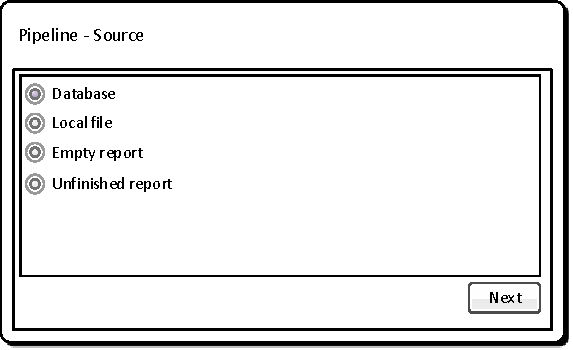
\includegraphics{Images/MockupPipelineSource}
        \caption{Selecting source of the report.}
        \label{fig:MockupPipelineSource}
\end{figure}

\begin{figure}[!htb]
        \centering
        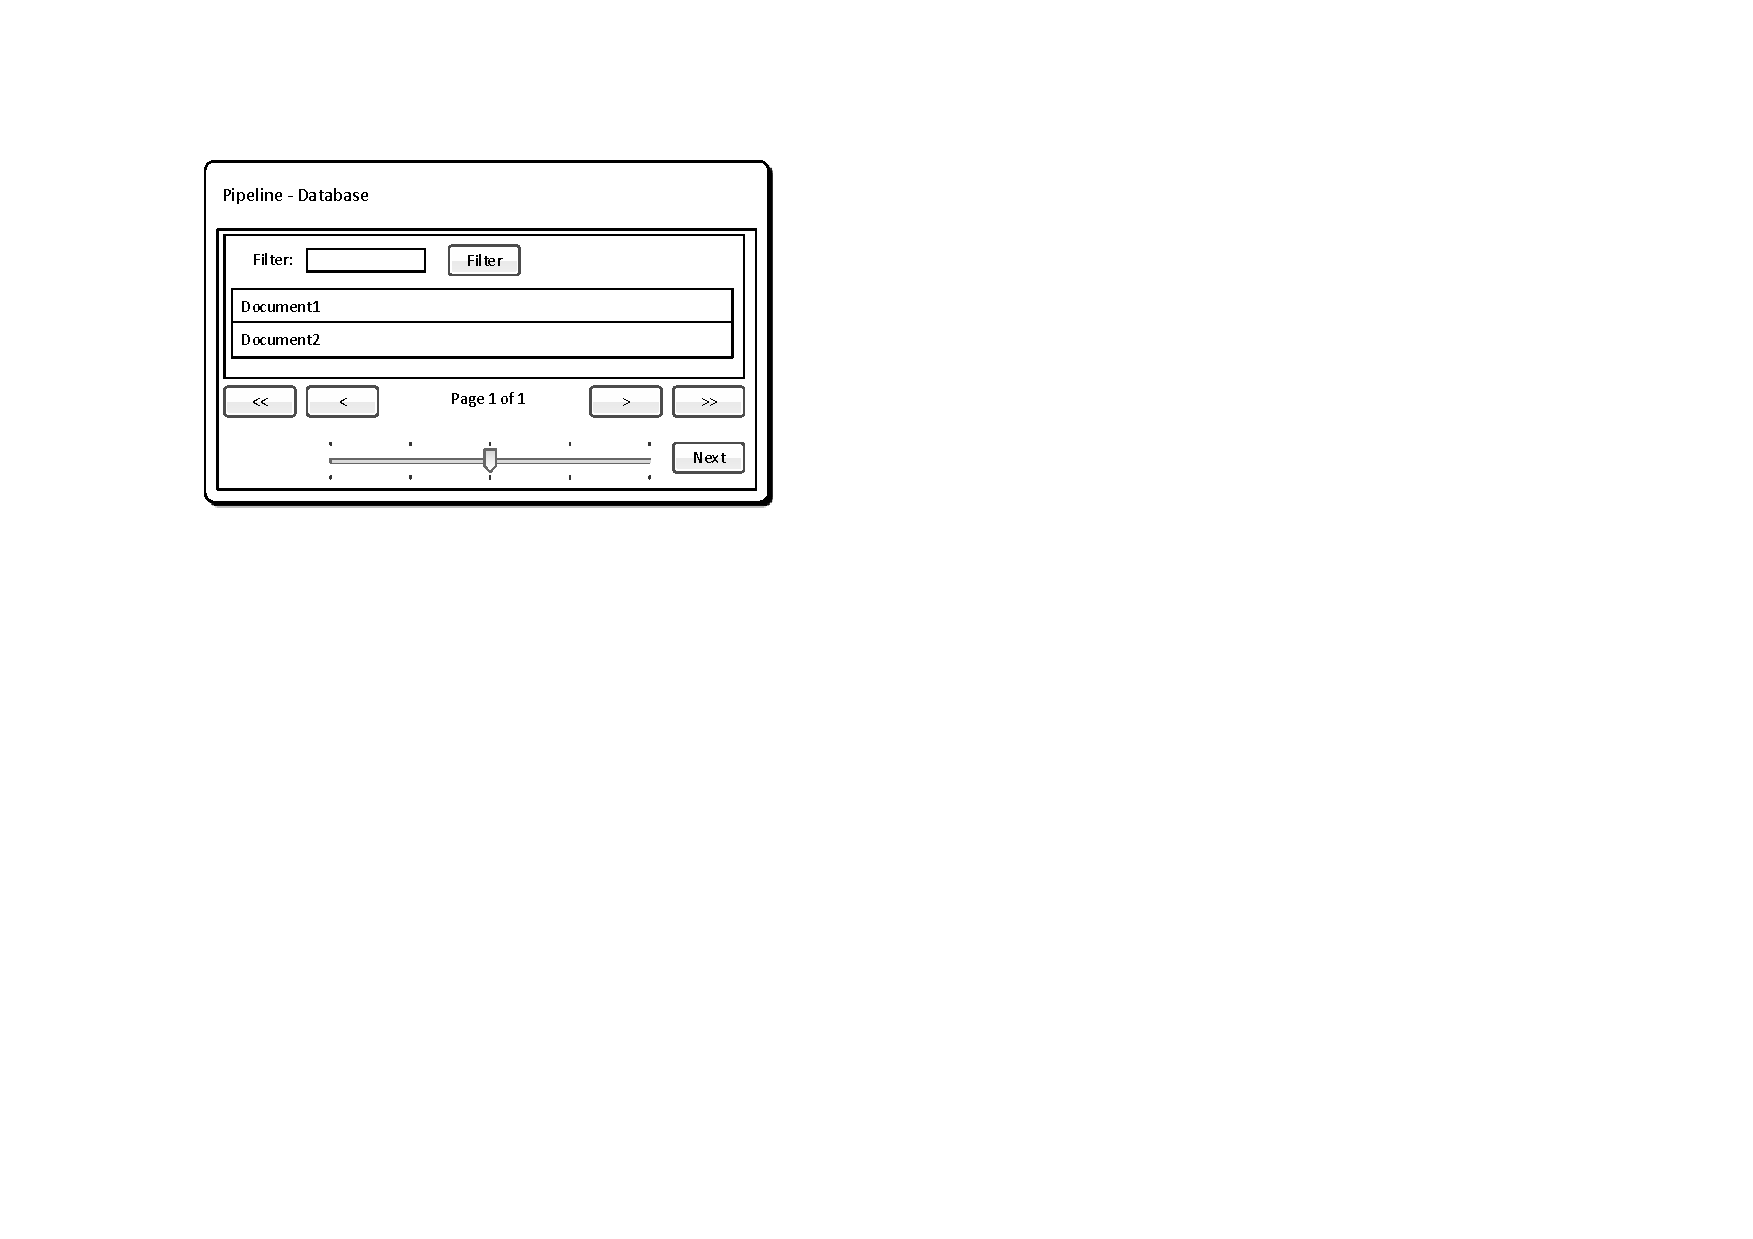
\includegraphics{Images/MockupPipelineDatabase}
        \caption{Selecting source of the report.}
        \label{fig:MockupPipelineDatabase}
\end{figure}

\begin{figure}[!htb]
        \centering
        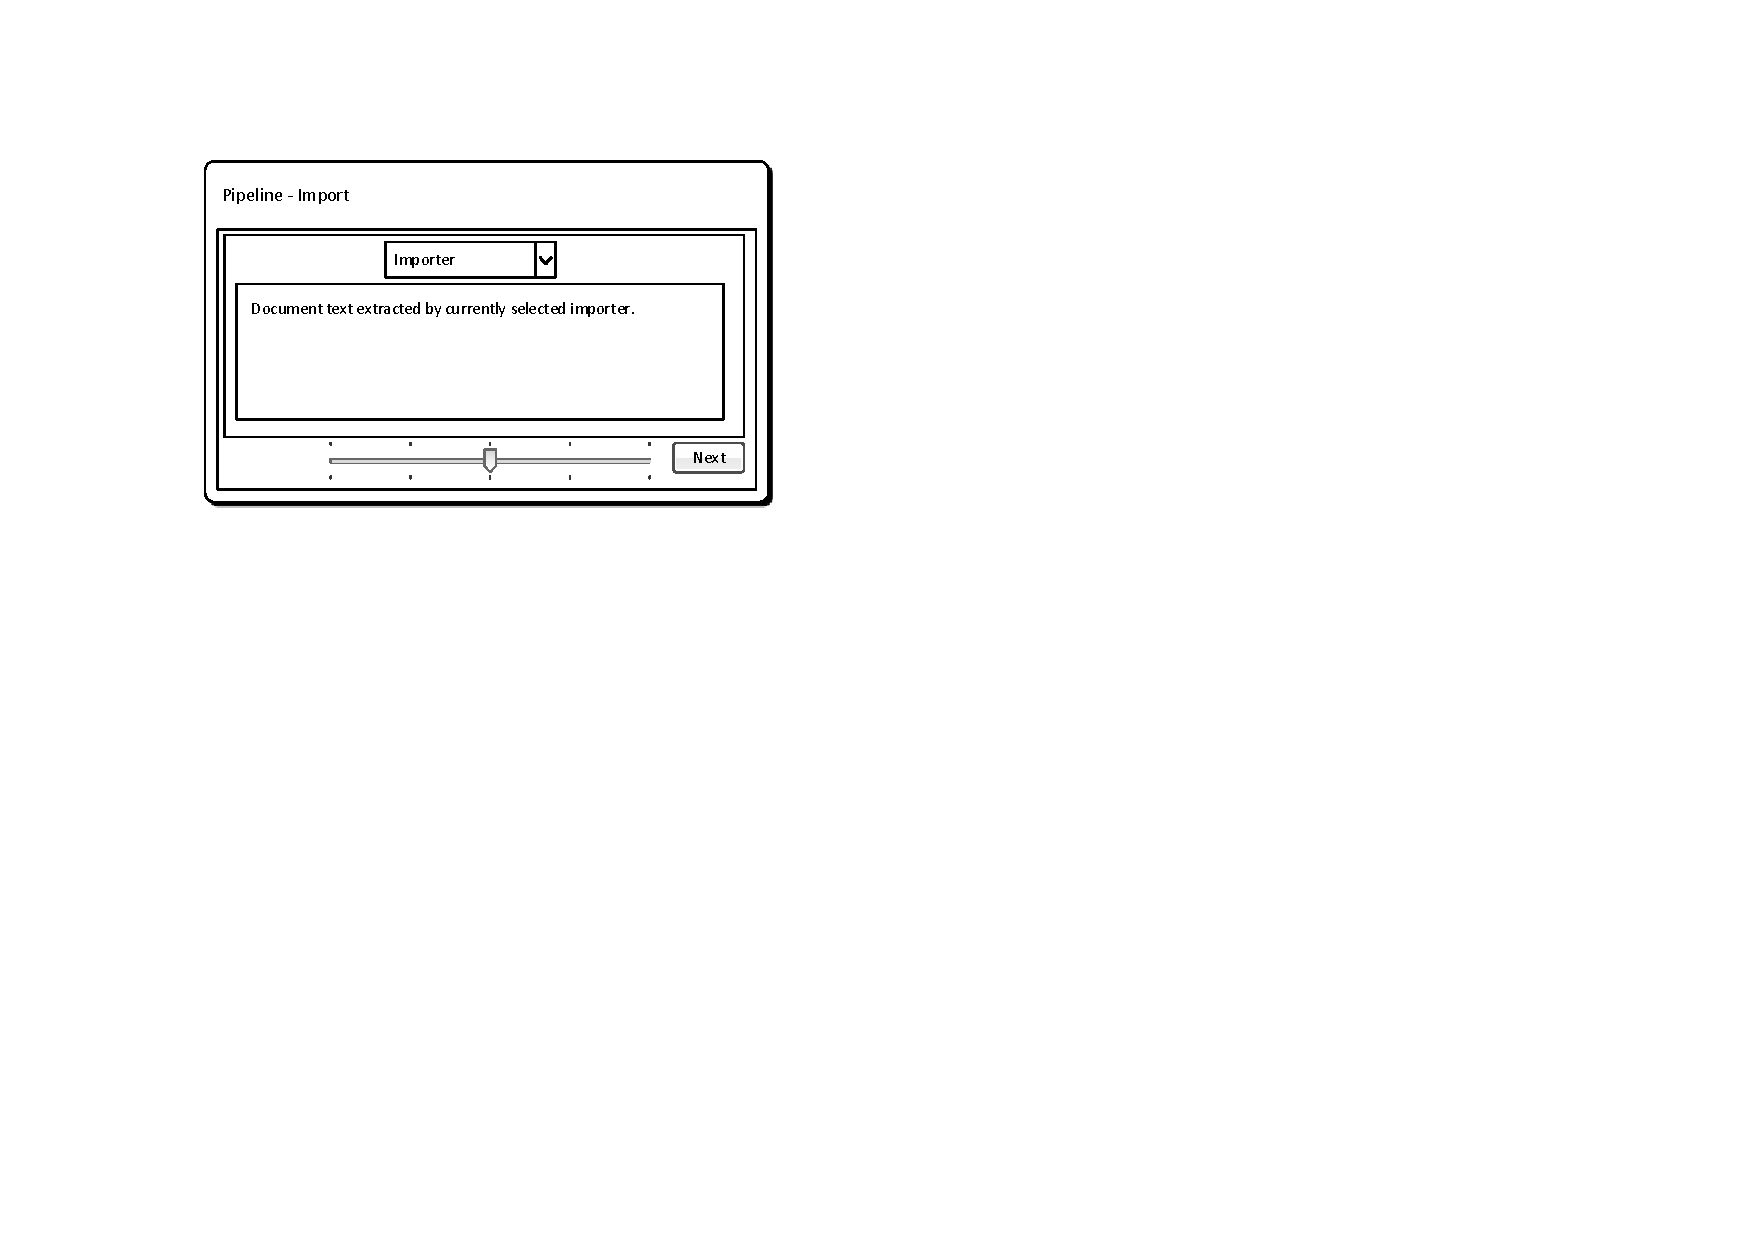
\includegraphics{Images/MockupPipelineImport}
        \caption{Importing report from a local file.}
        \label{fig:MockupPipelineImport}
\end{figure}

\begin{figure}[!htb]
        \centering
        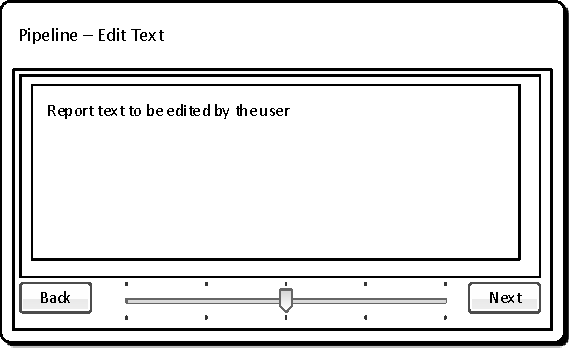
\includegraphics{Images/MockupPipelineText}
        \caption{Editing report text.}
        \label{fig:MockupPipelineText}
\end{figure}

\begin{figure}[!htb]
        \centering
        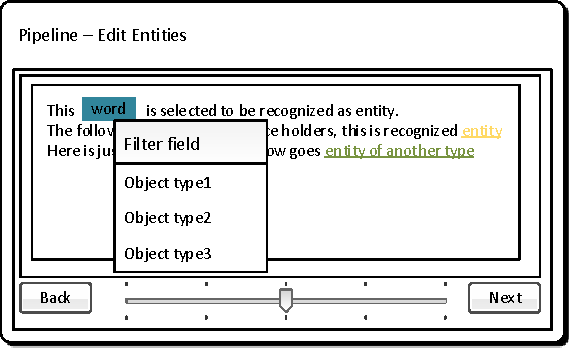
\includegraphics{Images/MockupPipelineEntities}
        \caption{Editing report entities.}
        \label{fig:MockupPipelineEntities}
\end{figure}

\begin{figure}[!htb]
        \centering
        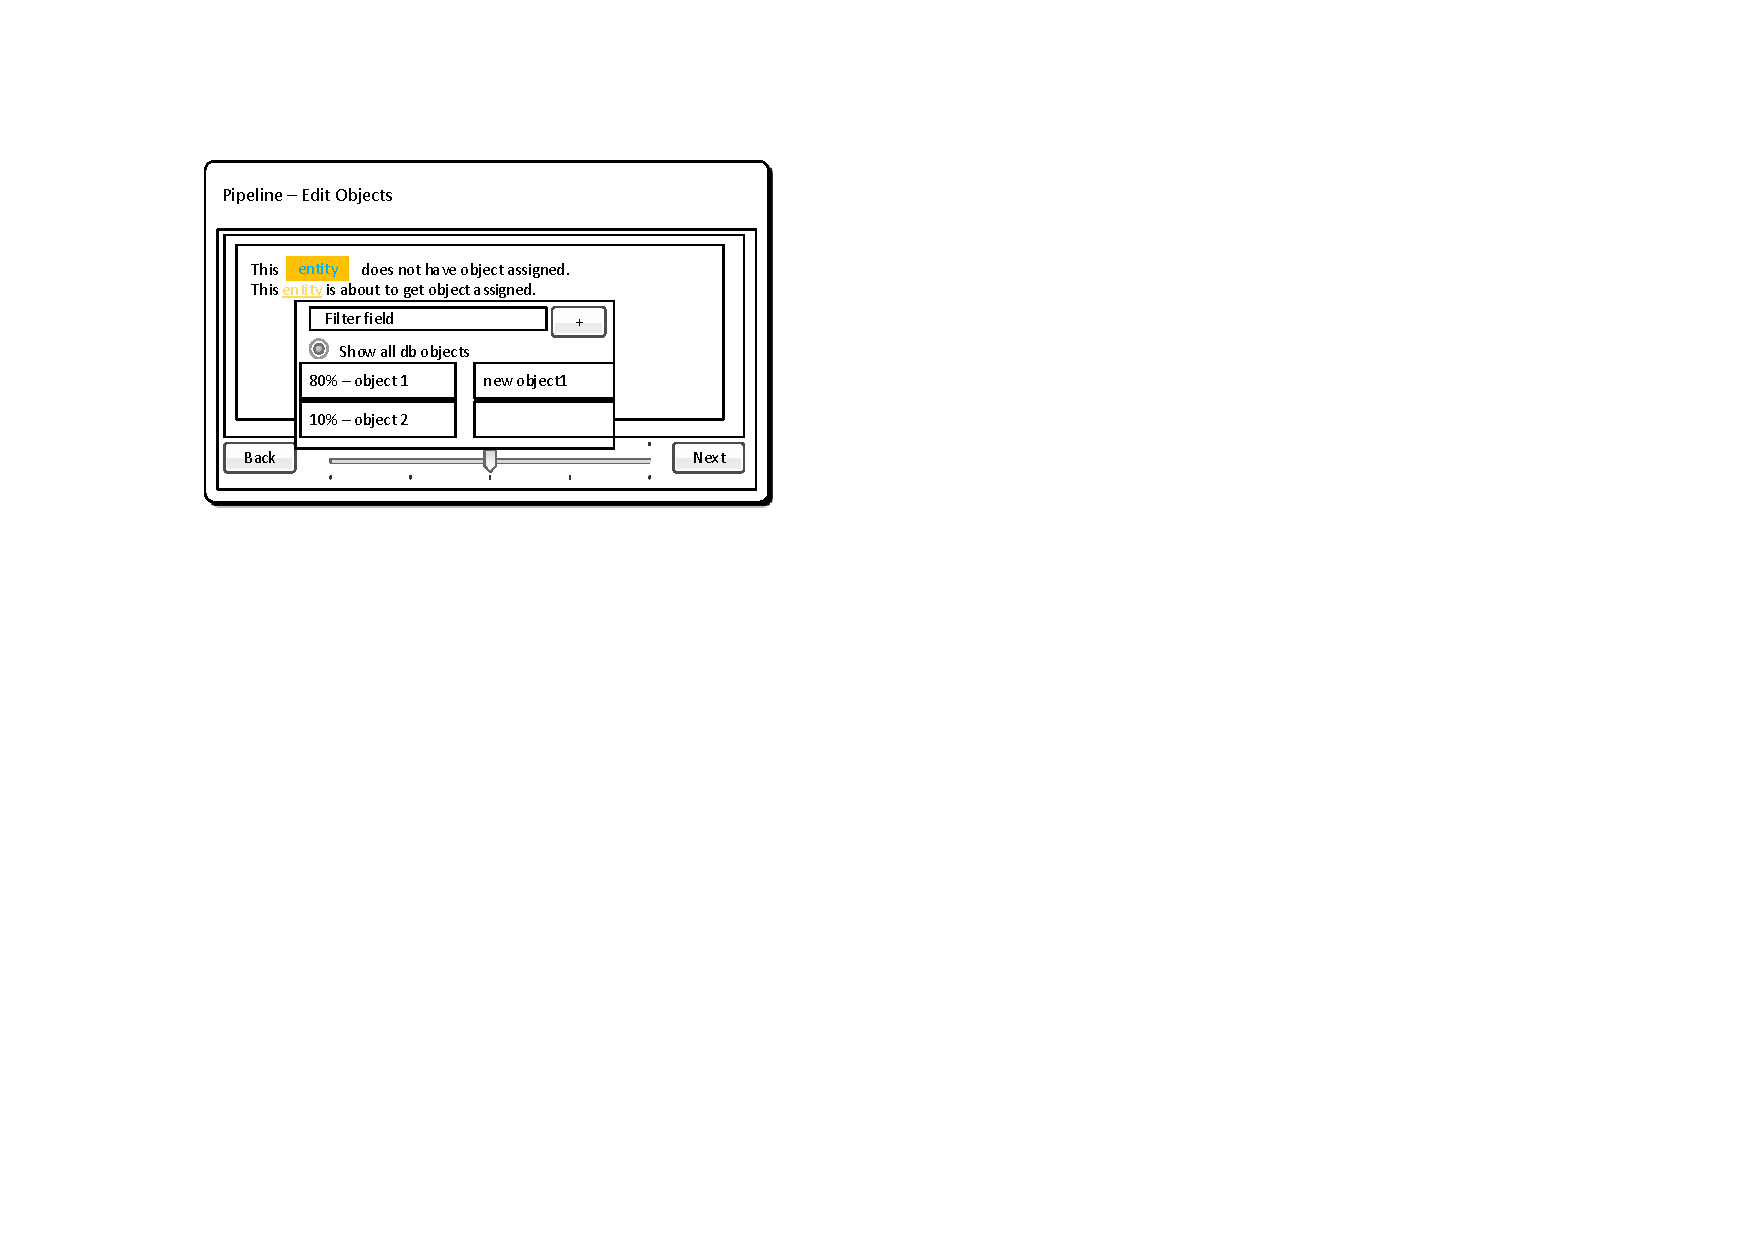
\includegraphics{Images/MockupPipelineObjects}
        \caption{Editing report objects.}
        \label{fig:MockupPipelineObjects}
\end{figure}

\begin{figure}[!htb]
        \centering
        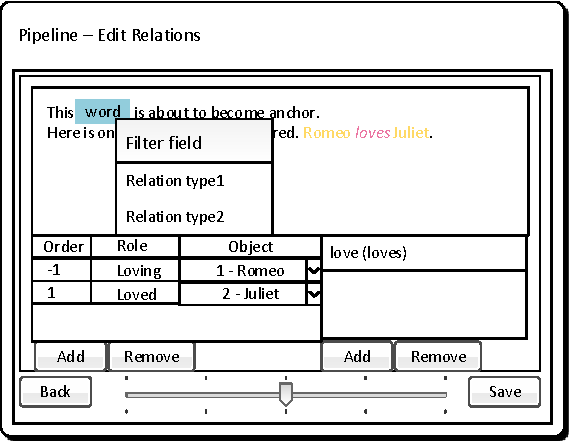
\includegraphics{Images/MockupPipelineRelations}
        \caption{Editing report relations.}
        \label{fig:MockupPipelineRelations}
\end{figure}

\begin{figure}[!htb]
        \centering
        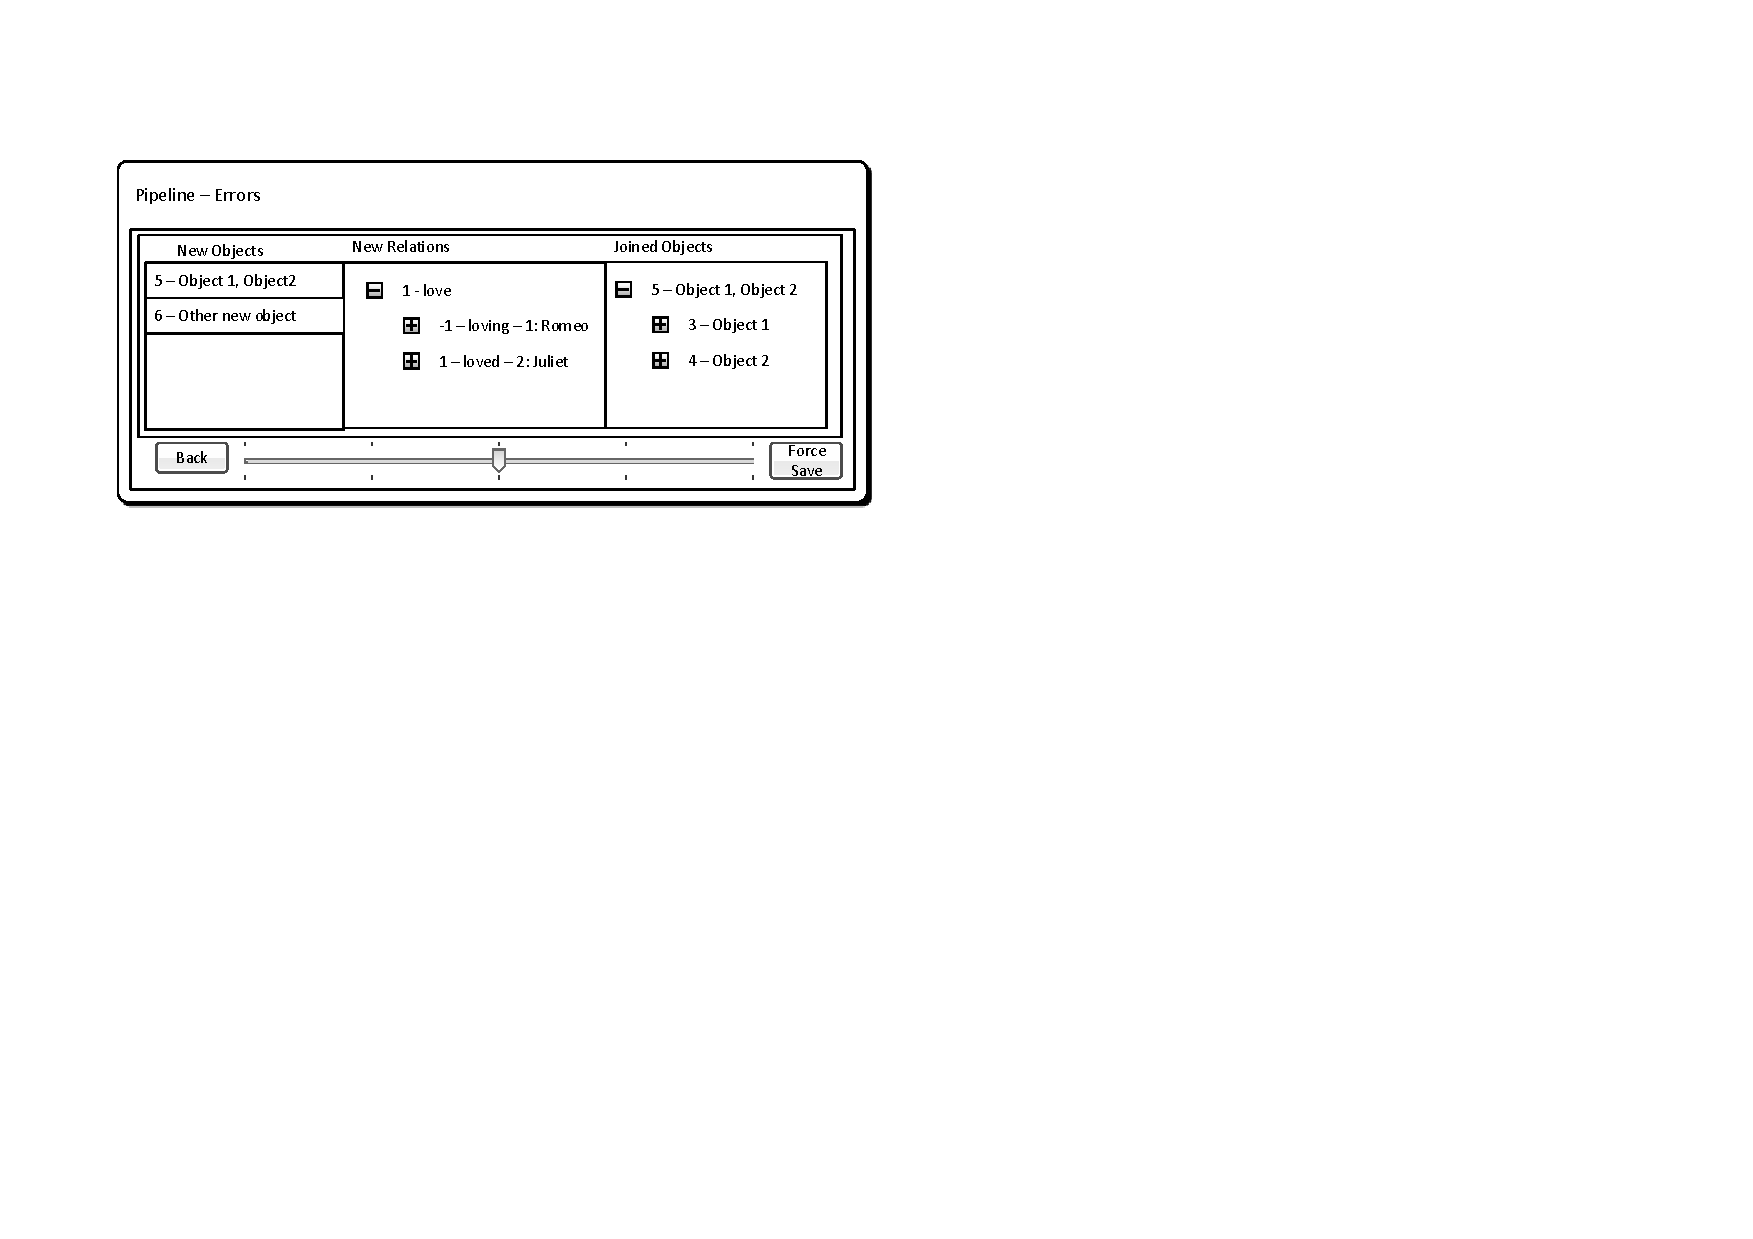
\includegraphics{Images/MockupPipelineErrors}
        \caption{Problems that may be detected on report saving.}
        \label{fig:MockupPipelineErrors}
\end{figure}

\subsection{Stateless or Stateful Communication}

Because part of processing is done on the server side and part in the client, it
is needed to somehow handle a state of processing. This problem is mostly solved
by sessions on server side. This approach has one disadvantage which is timeout.
Sessions cannot be easily implemented without any timeout due to their life cycle.

The main problem with sessions in \textan{} is that documents are processed mainly
by human users which can take a long time, especially when an unfinished processing
of a document can be saved on the client side. Due to this problem, any timeout
cannot be used.

We decide to solve this problem by storing whole state on client side when it is
necessary. It allows the server to be stateless. This approach has also some
disadvantages, for example that bigger messages are transferred over a network.
%Another big disadvantage is security.

\subsection{Database}

First problem we had to face was choosing the type of database. We considered
both relational and \emph{NoSQL} databases because we need both sequential
access and graph operations. The optimal solution would be using some kind of
hybrid database, however the support of relational databases is much better
and sequential access is a little more important for our use case, so we decided
to use relational database. In such database exact schema must be known and any
further changes in it can be very hard to perform in already running
system. On the other hand, relational databases are more type safe. There can be
constraints on columns that secure meaningful information in the records. Graph
databases basically look like a graph - there are nodes and edges, both can have
any additional information of any kind. These are suitable especially for graph
queries that cannot be done easily in relational databases.

To sum our reasons for preferring relational databases over graph databases, the
graph databases are pretty new technology, it is not so time proven and we
were too afraid of possible bugs. Apart from that relational database are well
documented, all main bugs have been solved years ago and everyone knows what to
expect and what is impossible.
We also wanted to use the database for machine learning, which uses sequential
access to the database. That is, as we know, faster in relational database,
where we can only iterate through all records in a single table.
And finally none of us have an experience with graph databases.

Although we have used relational database, this decision can be proven wrong and
through the time it can come out that graph database can be much better
solution. To deal with this possibility we have used the DAO design pattern
enabling to change the type of database without changing the application source
code. This pattern is more described in Section \ref{sec:PersistentLayer} about
server architecture respectively persistent layer.

Although this project is inspired by the Police and their reports with a
very specific domain, we decided to create a domain-independent model. This
allows easy transfer to other domains so the project could become wide spread
text recognizer solution. The model is described in details in Section
\ref{sec:Database} about the database.

\subsection{Adding New Object/Relation Types}
\label{ssec:AddingTypes}

We decided that only administrators are allowed to add new object and relation
types. This is because there should be a convention used by all users that could
be ruined by uncontrolled type explosion. Limiting types manipulation should
enforce that all interventions are well thought and conceptual.
